\chapter{Resultaten}
Dit hoofdstuk omvat de deel 2 en 3 van de onderzoekscyclus beschreven in \textit{Wat is Onderzoek?} (zie figuur \ref{fig:VerzamelEnAnalyseerCyclusen}).
Dit wordt gedaan door de vragen te beantwoorden van hoofdstuk \ref{chap:Onderzoeksopzet}.
Dit hoofdstuk is opgedeeld in de verschillende deelvragen waarbij in elk hoofdstuk een andere deelvraag wordt besproken.

\begin{graphic}
	\vspace{0.2cm}
	\captionsetup{type=figure}
    \caption{Deel 2 en 3 van de onderzoekscylcus afgeleid van \textit{Wat is Onderzoek?}}
    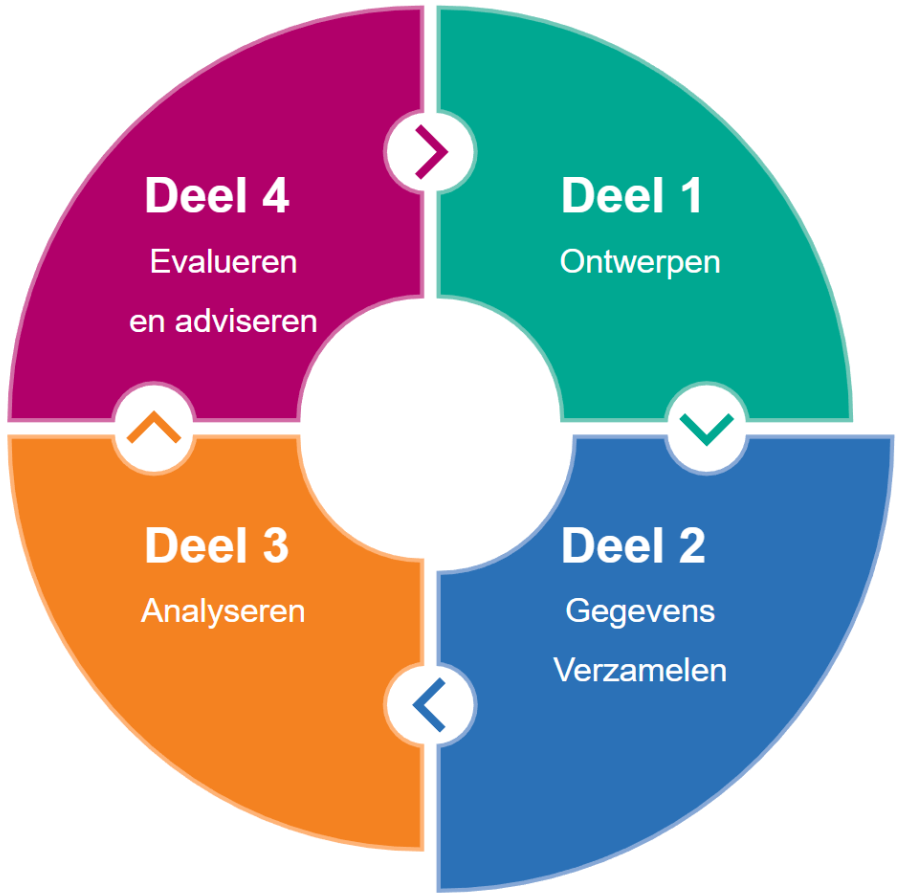
\includegraphics[scale=0.4]{img/GegevensVerzamelenCyclus.png}
	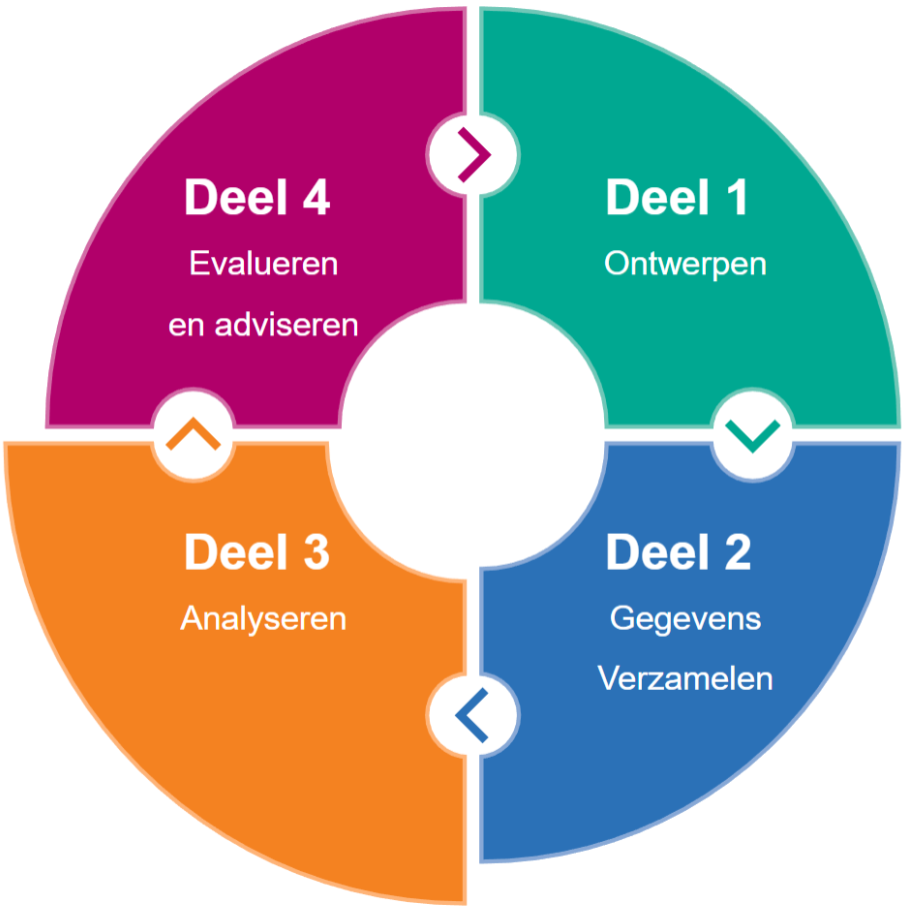
\includegraphics[scale=0.4]{img/AnalyserenCyclus.png}
		\label{fig:VerzamelEnAnalyseerCyclusen}
	\vspace{0.2cm}
\end{graphic}

\newpage
\section{Deelvraag 1: Stakeholders}
\label{sec:Stakeholders}
De stakeholders zijn individuen of organisaties die invloed of belang hebben bij het project.
Er is voor gekozen om de product owner als representatie te gebruiken voor de kleine bedrijven.
Dit is gedaan omdat het project nog in een proof of concept fase is en Snakeware hier nog geen klanten wil bij betrekken.
% Sommige externe stakeholders zullen gerepresenteerd worden door een gekwalificeerde interne medewerker van Snakeware.
% Dit wordt gedaan omdat de afstudeeropdracht een proof of concept is, en de klanten van Snakeware hier nog niet bij betrokken worden.
Als na de afstudeerperiode het een succes blijkt te zijn en Snakeware wil het verder ontwikkelen dan wordt contact opgezocht met de externe stakeholders (potentiële kleine bedrijven).
Er is een invloed matrix gemaakt (figuur \ref{fig:StakeholdersInvloedMatrix}) om de invloed en belang van de stakeholders te visualiseren.
Het project bestaat uit de volgende stakeholders:

\whitespace
\textbf{CEO:}
CEO Hans Hoomans is een van de oprichters van Snakeware en is verantwoordelijk (samen met de andere directieleden) voor de toekomstvisie van Snakeware.
Tijdens het opstellen van de opdracht is al aangegeven dat Hans veel ideeën heeft voor een nieuw \gls{CMS} als een product onder Snakeware.
Hierom is besloten om hem mee te nemen in het project om de toekomstvisie te integreren in het project.

\whitespace
\textbf{Product Owner:}
De product owner Elsa Croes is een projectmanager van de huidige kleine bedrijven die Snakeware heeft.
Samen met de product owner wordt de progressie bijgehouden van het project, en tijdens de realisatiefase wordt de progressie gepresenteerd.
Dit wordt gedaan om te zien of het project nog op het goede pad is en mogelijk bij te sturen als de wensen van de stakeholders veranderen.

\whitespace
\textbf{Kleine bedrijven:}
De kleine bedrijven zijn de eindgebruikers van het project, hierom is het van belang om hun eisen en wensen mee te nemen in het proces.
Het project is een proof of concept hierom is ervoor gekozen om de huidige kleine klanten niet direct betrekken bij het realiseren van het systeem.
Om toch een representatie te hebben van de kleine bedrijven is er gekozen om de product owner gebruiken als gekwalificeerde medewerker om de kleine klanten te vertegenwoordigen.% De medewerker die de kleine bedrijven representeert is Elsa Croes, zij is de productmanager van de huidige kleine bedrijven die Snakeware heeft.
De kleine bedrijven worden gebruikt als stakehoders om de gewenste functionaliteiten in beeld te brengen.

\whitespace
\textbf{Afdeling R\&D:} De afdeling R\&D van Snakeware zijn de ontwikkelaars van het huidige \gls{CMS} en kunnen veel inzicht bieden in de huidige situatie / problemen.
Tijdens de realisatie en ontwerpfase kan er advies gevraagd worden aan de backend en frontend developers van het R\&D team.
Na de afstudeerperiode wordt het project overgedragen aan het R\&D team.

\begin{graphic}
	\captionsetup{type=figure}
	\caption{Stakeholders invloed matrix}
	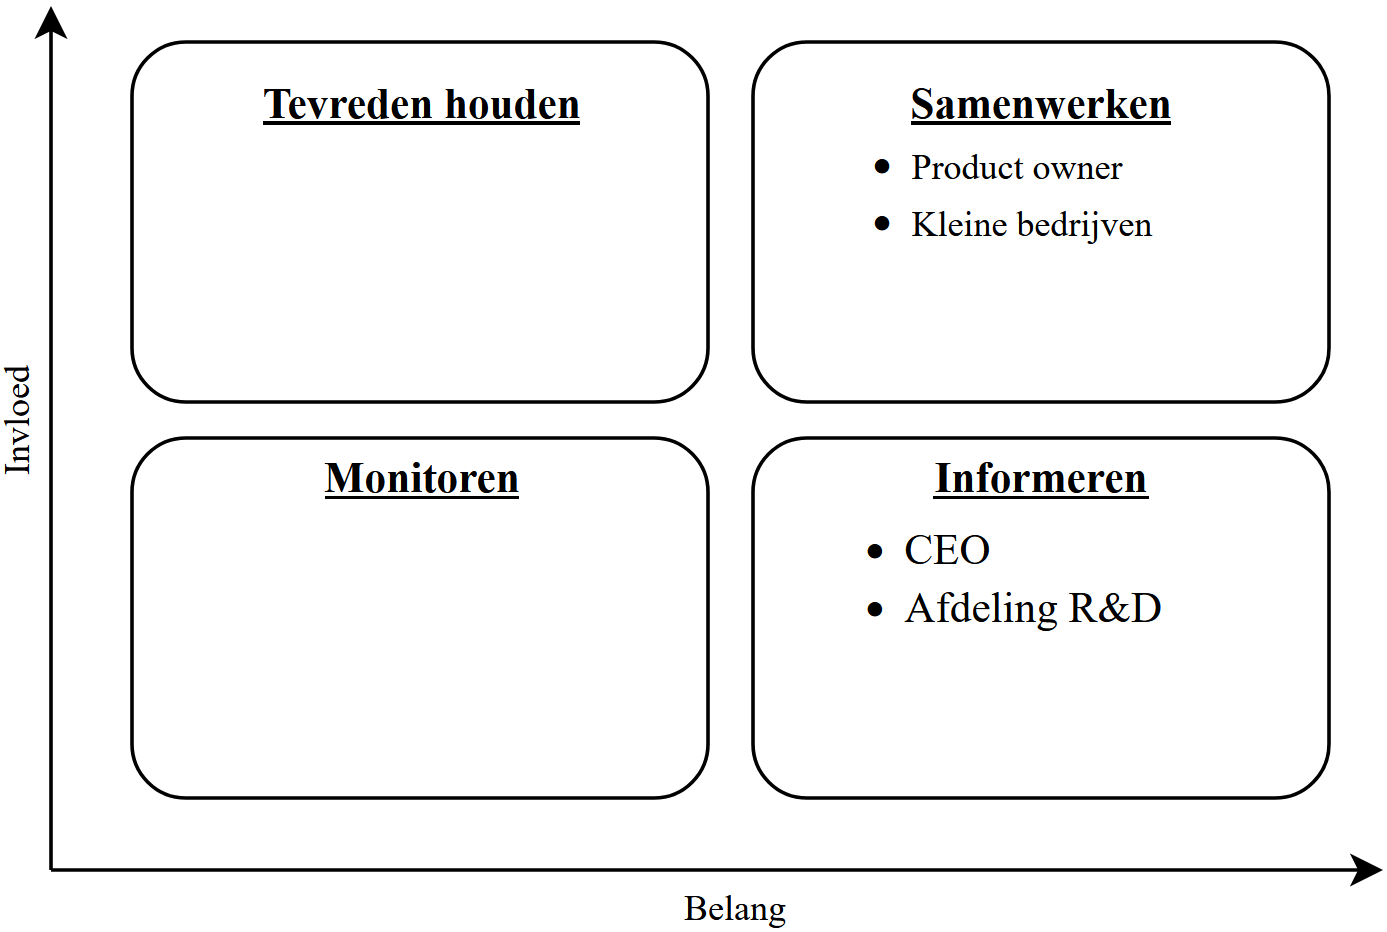
\includegraphics[scale=0.30]{StakeholdersInvloedMatrix}
	\label{fig:StakeholdersInvloedMatrix}
\end{graphic}

% \todo[inline]{Het stakeholder verhaal uitzoeken na dat de herfst vakantie (voor of kleine klanten er we of niet er tussen moeten staan).}
% \todo[inline]{De afbeelding klopt niet omdat hans er nog niet tussen staat en van wege het verhaal hier boven ik pas deze afbeelding aan als er bekend is wat er moet gebeuren met het verhaal hier boven.}
% \todo[inline]{Net zoals ik zei in methodologie, als ik de product owner ben zou elsa dan de representatie zijn voor de kleine klant? Dit is vaag }
% \todo[inline]{Als er woorden over zijn maak een kleine samenvatting voor het resultaat}

\newpage
\section{Deelvraag 2: Architectuur}
In deze paragraaf zijn de resultaten voor deelvraag 2 \qw{\textit{\SubquestionTwo}} verzameld en geanalyseerd.
Er is samen met de architect van het CMS Erwin Keuning en met software engineer Kevin Snijder een IT architecture sketching sessie gedaan.
In deze sessie is de huidige softwarearchitectuur inbeeld gebracht en is er ook aandacht besteed aan het in beeld brengen van het datamodel.
Verder is er ook gebruik gemaakt van interne documentatie van het systeem om de tekeningen te ondersteunen.
De diagrammen zijn afgeleid van de originele tekeningen die gemaakt zijn tijdens de sessie deze tekeningen zijn te vinden in Bijlage \ref{appendix:ITArchitectureSketch}.

\subsection{Systeem}
Het eerste gedeelte van de IT architecture sketching is besteed aan het in beeld brengen van het huidige CMS, en hoe het interacteert met de huidige sites die Snakeware onderhoud.
Snakeware heeft op dit moment 3 verschillende modellen aan websites die ze onderhouden \gls{XSL}, Vue 2 en Vue 3.

\whitespace
De \gls{XSL} site is het oudste website model dat Snakeware nu onderhoudt en maakt gebruik van de Snakeware Site code base.
Omdat origineel de \gls{XSL} sites er eerder was dan het \gls{CMS} was er des tijds voor gekozen om het van dezelfde Snakeware Site code base als basis te gebruiken.
% Dit heeft ervoor gezorgd dat het huidige \gls{CMS} aan te passen is met het \gls{CMS} (dit wordt alleen nooit gedaan).
De \gls{XSL} sites werken door middel van \gls{Stored procedures} om hun data op te halen en direct omzetten naar XML.
In figuur  \ref{fig:SystemArchitectureXSL} is te zien hoe de communicatie is tussen de verschillende systemen.
% Het eerste gedeelte van het IT Architecuture sketching is besteed aan het globale systeem / flow van het systeem.
% Er zijn op dit moment 3 verschillende Snakeware Cloud site methodes deze methodes zijn \gls{XSL} \Parencite{XSL}, Vue 2 en Vue 3 \Parencite{Vue} site.
% De Vue 2 en 3 werken door middel van de Snakware Cloud API en de \gls{XSL} werkt door middel van de Snakeware.Site code base.
% In afbeelding \ref{fig:SystemArchitectureXSL} is te zien hoe de \gls{XSL} sites werken, in afbeeldingen \ref{fig:SystemArchitectureVue} is te zien hoe de vue sites werken.
%
% \whitespace
% Het Snakeware Cloud platform zelf is een \gls{XSL} site dat aangepast kan worden door middel van het CMS (dit wordt alleen nooit gedaan).
% Er wordt gebruik gemaakt van stored procedures om de data op te halen van de database, deze data wordt automatisch omgezet naar XML.
% De XML wordt getransformeerd in bruikbare JSON format \Parencite{JSON} in het geval van de Vue 2 en 3 sites, en in het geval van een \gls{XSL} site wordt het getransformeerd naar javascript en HTML \Parencite{HTML}.
% deze data wordt vervolgens gebruikt om de data te tonen op de frontend.
%

\whitespace
\begin{graphic}
	\captionsetup{type=figure}
	\caption{Globale systeemarchitectuur \gls{XSL} sites}
	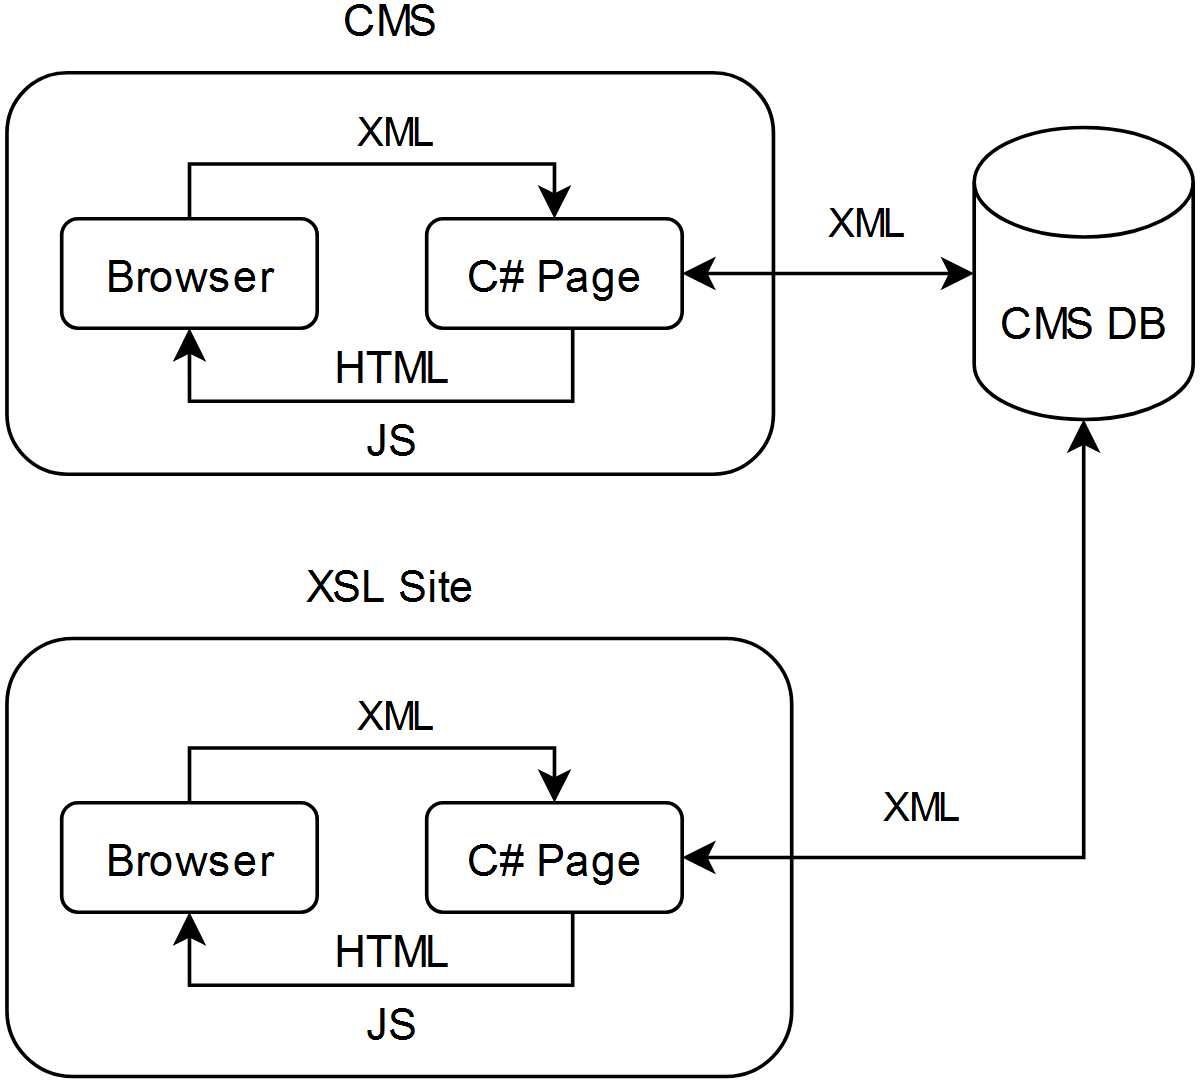
\includegraphics[scale=0.4]{XSLCMS}
	\label{fig:SystemArchitectureXSL}
\end{graphic}

\newpage

\whitespace
In het geval van de Vue sites wordt de XML omgezet naar het JSON format \parencite{JSON}.
Deze JSON wordt weer gebruikt om de correcte data te tonen op de frontend.
Een representatie van de flow van de Vue sites is te zien in figuur \ref{fig:SystemArchitectureVue}

\begin{graphic}
	\captionsetup{type=figure}
	\caption{Globale systeemarchitectuur Vue 2 en 3 sites}
	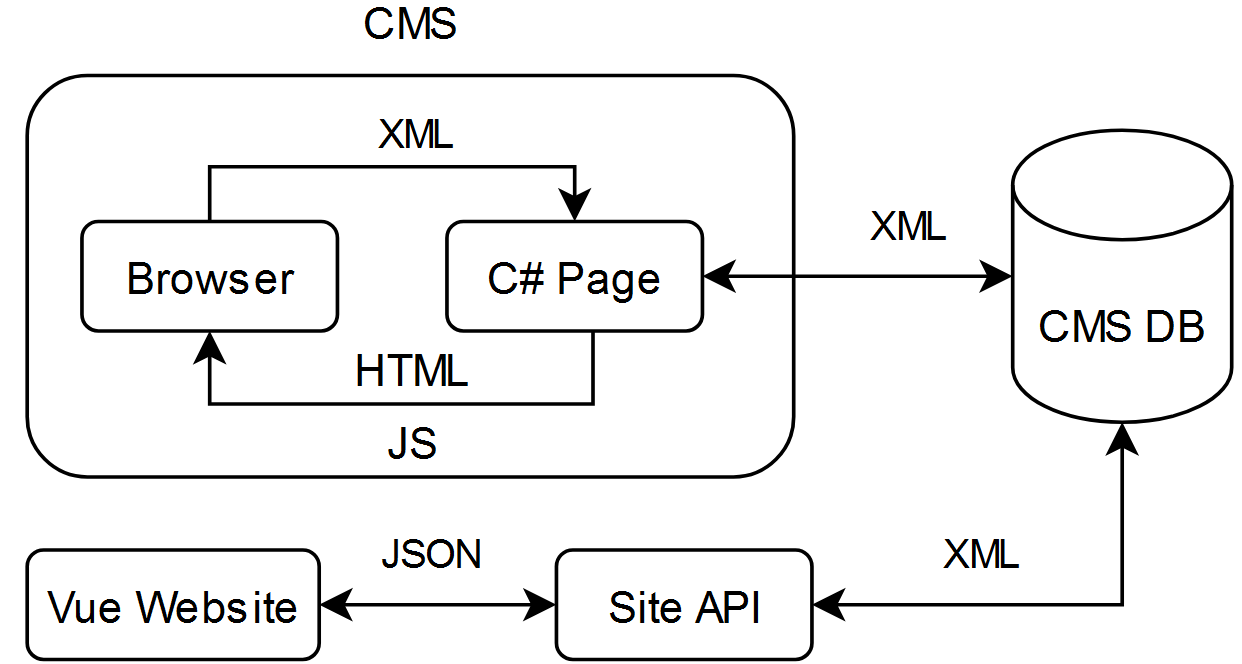
\includegraphics[scale=0.4]{VueCMS}
	\label{fig:SystemArchitectureVue}
\end{graphic}

% \todo[inline]{Ik had het ook nog even aan Stefan gevraagd en die zijn dat het prima is omdat het een representatie is van de tekeningen}

\whitespace
Tijdens de IT architecture sketching was er ook ruimte overgelaten om te onderzoeken waar er mogelijk verbeteringen gemaakt konden worden.
Uit de persoonlijke communicatie met Erwin en Kevin zijn de volgende punten uit gekomen.

\begin{itemize}
	\item[-]{Het Huidige \gls{CMS} maakt geen gebruik van de SOLID principes, dit zorgt ervoor dat het moeilijk te testen en uit te breiden is van wege de interconnected code}
	\item[-]{Het \gls{CMS} is op dit moment een grote monoliet, dit brengt problemen met zich mee rond het schalen en onderhouden van het systeem.
	      Dit lukt op het moment niet door de interconnected code van het CMS.}
	\item[-]{Het is momenteel niet realistisch om het \gls{CMS} te testen door middel van unit testen, dit is echter wel gewild.}
	\item[-]{Veel van de logica van het CMS zit vastgekoppeld in de frontend, en dit is niet gewild.
	      Dit levert nu veel problemen op met het onderhouden van het CMS.}
\end{itemize}

\newpage
\subsection{Het datamodel}
\label{subsection:Datamodel}
Het volgende onderdeel is het schetsen van het datamodel, dit is ook gedaan samen met Erwin en Kevin.
Op dit moment maakt het \gls{CMS} gebruik van 288 tabellen, deze tabellen bevatten meerdere kolommen en zijn interconnected.
Daarom is er tijdens het schetsen van het datamodel alleen gekeken naar de belangrijkste tabellen en de relaties hiertussen.
De exacte data dat opgeslagen wordt in deze tabellen weggelaten om het overzichtelijk te houden.
Het versimpelde datamodel van het CMS is te zien in figuur \ref{fig:DatamodelCMS}.

\whitespace
\begin{graphic}
	\captionsetup{type=figure}
	\caption{Gesimplificeerde datamodel CMS}
	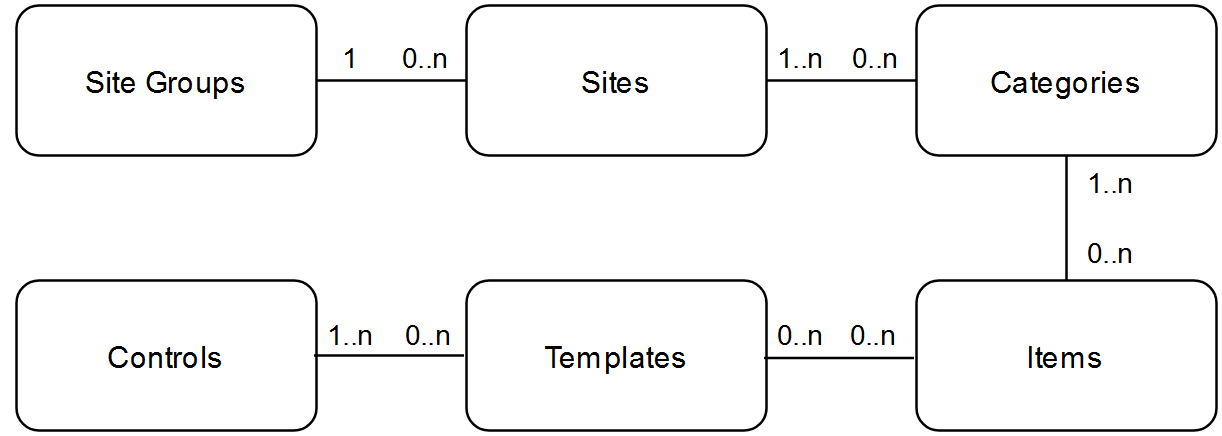
\includegraphics[scale=0.45]{CMSDatabaseModelB}
	\label{fig:DatamodelCMS}
\end{graphic}

\whitespace[2]
Na het schetsen van het datamodel is er gevraagd waar op dit moment de meeste problemen worden gevonden in het datamodel.
Deze punten zijn verzameld tijdens de sessie door middel van persoonlijke communicatie met Erwin en Kevin.
\begin{itemize}
	\item[-]{Het datamodel is erg complex, dit maakt het lastig om nieuwe functionaliteiten in het CMS te bouwen}
	\item[-]{Het datamodel heeft te veel connecties met andere tabellen terwijl dit niet nodig zou moeten zijn.
	      Dit maakt het systeem onnodig complex.}
	\item[-]{De huidige naamgeving van de tabellen en kolommen is niet als gewild.
	      Als dit nu aangepast zou worden zou dit voor veel problemen opleveren in de code, maar met een nieuw project is het gewild dat er een andere naamgeving wordt gebruikt.}
\end{itemize}
% \todo[inline]{dit denk ik weg halen}
% Tijdens de sessie kwam er naar voren dat mensen binnen het R\&D uitgesproken meningen hebben over een nieuw datamodel.
% Hierom wordt er tijdens de ontwerpfase met het R\&D team een sessie gepland om ideeen te leveren voor een nieuw data model.
% Deze input zal gebruikt worden om het datamodel te ontwerpen.
%

\subsection{Antwoord en resultaat}
Samen met Erwin Keuning en Kevin Snijder zijn er door middel van IT architecture sketching 2 systeem schetsen gemaakt (zie figuur \ref{fig:SystemArchitectureXSL} en \ref{fig:SystemArchitectureVue})
Door middel van deze tekening is het huidige systeem en datamodel (zie figuur \ref{fig:DatamodelCMS}) in beeld gebracht.
Daarnaast zijn er door de gesprekken met Erwin en Kevin de volgende randvoorwaarden opgesteld.

\begin{itemize}
	\item[-]{Het eindproduct moet aan de documentatie standaarden voldoen van Snakeware.}
	\item[-]{Het eindproduct moet gebruik maken van moderne codering best practices (bijvoorbeeld SOLID)}
	\item[-]{De code moet voldoen aan huidige coderingsstandaarden}
	\item[-]{De code moet getest worden door unit en integratie tests.}
    \item[-]{De code zal geschreven worden in C\# \Parencite{CSharp} en in Typescript \Parencite{Typescript}.}
\end{itemize}


\newpage
\section{Deelvraag 3: Knelpunten}
In dit hoofdstuk worden resultaat van deelvraag 3 \qw{\textit{\SubquestionThree}} verzameld en geanalyseerd.
Voor deze deelvraag zijn er 2 expertinterviews gedaan met Janny Reitsma en Rob Douma.
Het interview met Janny is uitgevoerd op 31 oktober 2023 en het interview met Rob op 2 november 2023.
In de volgende subsecties de belangrijkste punten van de interviews genoemd en behandeld.
De interviews zijn opgenomen en zijn transcripties van gemaakt die te vinden zijn in bijlage \ref{appendix:ExpertInterviews}

\subsection{Janny Reitsma interview}
\label{sec:JannyInterview}
Janny Reitsma werkt voor de service desk van Snakeware, en geeft cursussen aan nieuwe klanten die het CMS gaan gebruiken.
Verder handelt Janny ook vaak de vragen en functionaliteit aanvragen van klanten af voor het CMS.

\whitespace
Tijdens het interview kwam het naar voren dat Janny vindt dat \gls{SEO} erg belangrijk is voor het CMS en dat het nu nog niet optimaal wordt afgehandeld.
Klanten kunnen in het huidige CMS artikelen linken naar andere plekken op hun site.
Helaas komt het vaak voor dat klanten linken naar verkeerd pagina's waardoor ze vaak bij de service desk komen om dit op te lossen.
% Klanten kunnen op dit moment vaak fouten maken door verkeerd pagina's te linken aan elkaar waardoor het niet altijd goed gaat.
Voor sommige \gls{SEO} tools moeten er elementen in de applicatie geplaatst worden.
Bij deze elementen kun je denken aan zogenaamde Facebook pixel \Parencite{FacebookPixel}.
Dit moet nu worden gedaan door een developer, dit kost tijd en geld hierdoor wordt Snakeware een duurdere partij.

\whitespace
Dit probleem speelt zich nu ook voor bij het integreren van derde partijen integraties.
Bij deze integraties kun je denken aan een cadeaubon widget of een kalender planner.
Het liefst wil Snakeware dat de klant dit zelf kan doen zodat Snakeware als goedkopere partij er uit komt.

\whitespace
Een andere groot punt is dat het huidige CMS interface niet meer van deze tijd is.
Het zou meer visueel moeten werken zodat klanten makkelijker kunnen zien waar hun content staat en hoe het getoond worden.

\subsection{Rob Douma interview}
\label{sec:RobInterview}
Rob Douma is een oud informatieanalist die in de loop der jaren naar een product owner rol binnen Snakeware veranderd.
Verder richt hij de functionele en technische kan van het CMS in voor de grotere klanten.

\whitespace
Tijdens het interview kwam het naar voren dat Rob redelijk tevreden is met de huidige functionaliteiten van het CMS. 
Hierbij werd vooral gesproken over de formulieren functionaliteit en de aanpasbaarheid van de artikelen.
Volgens Rob moet zulke functionaliteit blijven zodat de klant meer zelf kan doen.

\whitespace
Een van de problemen die Rob wel aankaartte, is dat het CMS nog te rigide voelt in hoe content geplaatst moet worden.
Rob zou graag een oplossing willen waar mee hij  de artikelen van de websites makkelijker kan beheren en groeperen.
Deze groepen zou hij graag weer kunnen gebruiken bij andere artikelen

% Hierdoor kost het soms meer tijd om content goed op de site te kunnen zetten.
% Een mogelijke oplossing hiervoor gaf Rob aan is het groeperen van content op basis van een container model.
% Waarbij je artikelen kan groeperen in een container en deze container kan injecteren in andere artikelen.
%
\newpage
\whitespace
Tijdens het interview is er ook gesproken over de huidige database structuur van het CMS.
Rob gaf aan dat er op dit moment veel legacy data in de database zit met alle gevolgen van dien.
Ook gaf Rob aan dat er veel logica in de database zit door middel van triggers en stored procedures, en dit is liever niet gewenst.

\subsection{Samenvatting en antwoord}
Er zijn twee interviewen gedaan met experts binnen Snakeware, deze experts waren Janny Reitsma en Rob Douma.
In het interview van Janny kwam naar voren dat een van de grote knelpunten is de huidige implementatie van \gls{SEO}.
Ook kwam er naar voren dat de klant meer zelf moet kunnen inrichten door middel van derde partijen integratie.

\whitespace
Bij het interview van Rob kwam naar voren dat de huidige knelpunten bij de flexibiliteit van het inrichten van content.
Rob gaf ook aan dat hij graag wil dat de flexibiliteit van artikeltypes en formulieren moet blijven.
Na dat de resultaten waren verzameld zijn de resultaten teruggelegd bij Janny en Rob.
Zij hebben de resultaten als juist beschouwd.

\newpage
\section{Deelvraag 4: Requirements}
\label{sec:Requirements}
In dit hoofdstuk worden de resultaten van deelvraag 4 \textit{\SubquestionFour} onderzocht.
Om met deze deelvraag te beantwoorden zijn er semigestructureerde interviews gehouden met de product owner en de CEO van Snakeware.
Tijdens de interviews wordt er gepraat over de eisen en wensen zodat deze in kaart kunnen worden gebracht.
Beide interviews zijn terug te vinden in bijlage \ref{appendix:ExploreUserRequirements}.

\subsection{Interview met Elsa Croes en Eric Dijkstra}
Het eerste interview wat plaats heeft gevonden is gedaan met de product owner Elsa Croes.
Om Elsa te ondersteunen en meer technisch kennis mee te nemen in het interview is er op het laatst moment een frontend developer mee genomen in het gesprek Eric Dijkstra.
Het interview heeft plaats gevonden op 6 november 2023 op locatie bij Snakeware.
Het interview begon met een kleine introductie wie ze zijn en wat ze doen binnen Snakeware.
Daarna zijn er eerst vragen gesteld om de kern functionaliteiten in beeld te krijgen en de eisen en wensen van de product owner.
Hier is er gesproken over een toekomstvisie van het systeem en de mogelijke functionaliteiten die zouden toegevoegd kunnen worden.

\whitespace
Er is ook gesproken over het belang van SEO in het proof of concept en hoe belangrijk dat dit geimplementeerd wordt.
Elsa en Eric gaven beide aan dat SEO erg belangrijk is voor een moderne site.
Zonder SEO-opties zou een site niet gebruikt kunnen worden door klanten omdat ze dan niet goed gevonden kunnen worden.
Het complete interview is te vinden in bijlage \ref{appendix:ExploreUserRequirementsElsa}.

\subsection{Interview Hans Hoomans}
Daarnaast is er ook interview gedaan met de CEO van Snakeware Hans Hoomans.
Het interview heeft plaats gevonden op 7 november 2023 op locatie bij Snakeware.
Tijdens het interview is erg van het originele pad afgegaan van de geplande vragen.
Er is vooral gesproken over een nieuw mogelijk datamodel en hoe dat impact zou hebben op het totale systeem.

\whitespace
Daarnaast is het een belangrijk voor Hans dat het PoC niet rigide aanvoelt.
Hans geeft aan dat een van de problemen waar Snakeware nu vaak tegen aanloopt, is dat er vaak een custom oplossing moet komen voor alle verschillende klanten.
Hij wil graag dat er meer generiek gewerkt wordt binnen Snakeware en dat software vaker hergebruikt kan worden. 
De quote waar Hans graag naar toe wil streven is \qw{kracht van eenvoud en herhaling}.
Dit zou hij graag terug willen zien in het datamodel door minder tabellen te gebruiken en meer generiek te werken.
Tijdens het interview is er vertrouwelijke informatie besproken dat Hans liever niet in de transcriptie wil hebben.
Hierom wordt er een samenvatting gemaakt van het interview deze samenvatting is te vinden in bijlage \ref{appendix:ExploreUserRequirementsHans}

\subsection{Antwoord en resultaat}
Na dat beide interviews waren afgenomen is er een lijst van user stories gemaakt.
Deze user stories zijn beide door Hans en Elsa als correct beschouwd.
In figuur \ref{fig:RequirementSimplified} zij de requirements te vinden.

\begin{graphic}
    \captionsetup{type=figure}
    \caption{Resultaat user requirements exploration}
    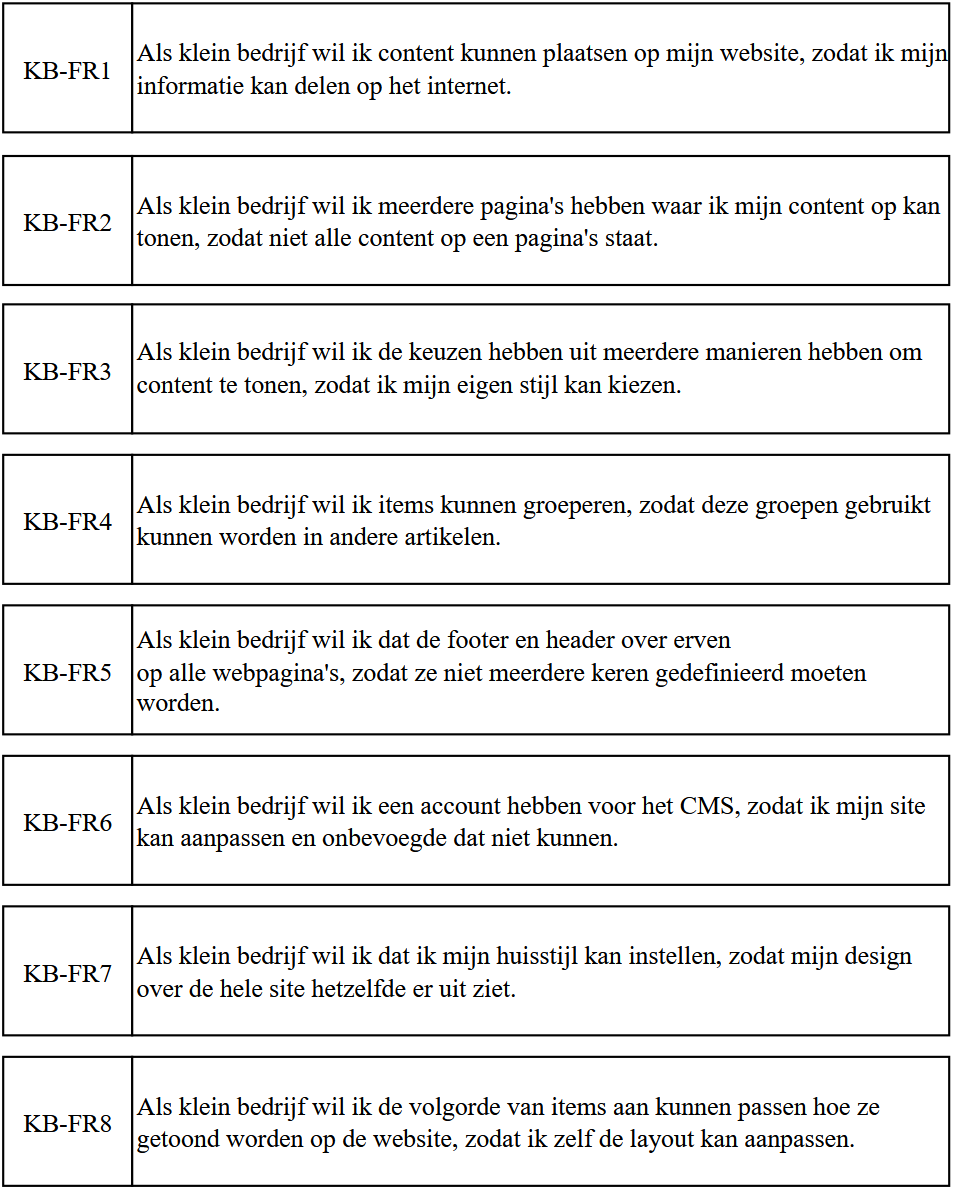
\includegraphics[scale=0.4]{FR1-8}

    \whitespace
    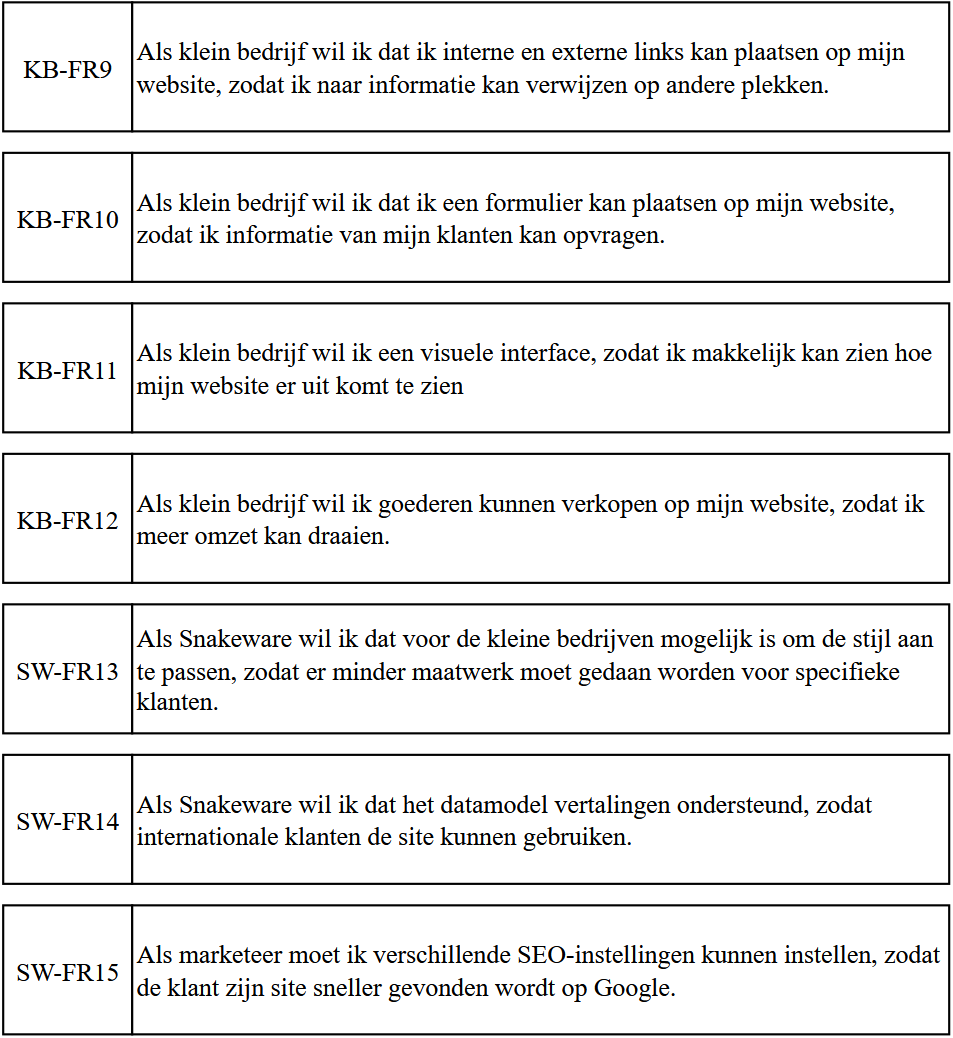
\includegraphics[scale=0.4]{FR9-15}
    \label{fig:RequirementSimplified}
\end{graphic}

\newpage
\section{Deelvraag 5: Prioritering}
\label{sec:Prioritering}
In dit hoofdstuk wordt de deelvraag beantwoord \qw{\textit{\SubquestionFive}}.
De requirements die uit deelvraag 4 zijn gekomen worden gecategoriseerd in 4 verschillende prioriteit niveaus.
Deze niveaus zijn bepaald door middel van de MoSCoW-methode \Parencite{MoSCoW}.
De MoSCoW-methode bestaat uit de volgende prioriteit niveaus:

\whitespace
\textbf{Must have:} Dit zijn de kern functionaliteiten, zonder deze functionaliteiten zou het project niet bruikbaar zijn en niet als succes beschouwd worden.

\whitespace[1]
\textbf{Should have:} Dit zijn de functionaliteiten die niet essentieel zijn maar wel belangrijke functionaliteiten toevoegen in het systeem.

\whitespace[1]
\textbf{Could have:} Dit zijn de functionaliteiten die je graag zou willen hebben.
Ze zijn niet essentieel als er tijd over is in het project zou je deze functionaliteiten realiseren.

\whitespace[1]
\textbf{Won't have:} Dit zijn de functionaliteiten die je zou willen zien in een ander stadium van een project.
Of als er tijd over is en al de andere functionaliteiten zijn al geïmplementeerd.

\whitespace[2]
Om de requirement te categoriseren in de categorieën van de MoSCoW-methode wordt er een score aan de requirement toe gewezen.
Deze score wordt bepaald door middel van formule \ref{eq:PioritizationRequirementsFormula}.
Deze formule komt origineel uit het onderzoeksverslag van Berber Bouma \Parencite{BerberVerslag}.
Voor dit onderzoek is alleen de requirement prioritering uit het verslag gebruikt.

\whitespace
\begin{equation}
	\label{eq:PioritizationRequirementsFormula}
	Score = TS + OS + (9 - duur)
\end{equation}

\whitespace
De formule bestaat uit de volgende aspecten:
\begin{enumerate}
	\item[-] Tevredenheidsscore (TS) [1,2,\ldots,5]: Deze waarden wordt toegekend door de stakeholder met betrekking van de requirement.
	      De stakeholder geeft een waarde van 1 tot 5 van tevredenheid als het geimplementeerd wordt.
	      Hierbij is een 1 niet erg tevreden en 5 erg tevreden.
	\item[-] Ontevredenheidscore (OS) [1,2,\dots,5]: Deze waarden wordt toegekend door de stakeholder met betrekking van de requirement.
	      De stakeholder geeft een waarde van 1 tot 5 van ontevredenheid als het niet geimplementeerd wordt.
	      Hierbij is een 1 niet erg onteverden en een 5 erg ontevreden.
	\item[-] Duur [1,2,3,5,8]: De duur representeert door een relatief getal om de geschatte tijd om de requirement te implementeren te representeren.
	      De waardes van de duur zijn een verkleinde selectie van Scrum poker \Parencite{ScrumPoker}.
	      Deze waardes worden geverifieerd door een senior developer zodat hier een correcte schatting van gemaakt kan worden.
\end{enumerate}

\whitespace
Het maximum wat doormiddel van deze formule behaald kan worden is 18 (5 + 5 + (9 - 1) = 18) en het minimum wat behaald kan worden is 3 (1 + 1 + (9 - 8) = 3).
Door het verschil van deze getalen te verdelen over 4 categorien krijg je de volgende getallen ranges:

\whitespace
\makebox[3cm][l]{Must have:} $ x \in \mathbb{R} : 14 \leq x \leq 18 $ \\
\makebox[3cm][l]{Should have:} $ x \in \mathbb{R} : 9 \leq x \leq 13 $ \\
\makebox[3cm][l]{Could have:} $ x \in \mathbb{R} :  5 \leq x \leq 8 $ \\
\makebox[3cm][l]{Won't have:} $ x \in \mathbb{R} : 3 \leq x \leq 4 $

\newpage
\subsection{Antwoord en resultaat}
Het resultaat van formule \ref{eq:PioritizationRequirementsFormula} en de categorisatie met behulp van de MoSCoW-methode is te zien in Tabel \ref{tab:RequirementPrioritization}.
De requirements zijn voorzien van een verwachte duur en acceptatiecriteria.
Een voorbeeld user story is te zien in tabel \ref{rq:res5Sample}.
Dit leidt tot 6 must have, 6 should have, 1 could have en 2 wont have requirements de volledige lijst met geprioriteerde requirements is te vinden in bijlage \ref{appendix:Requirements}.
Het resultaat van de deelvraag is terug gelegd bij de product owner en hebben de resultaten als juist beschouwd.

\begin{graphic}
	\vspace{0.2cm}
	\captionsetup{type=table}
	\caption{gepriotiriseerde requirement}
	\begin{tabular}{ |p{3cm}||p{1cm}|p{1cm}|p{1.5cm}|p{1cm}|p{2.5cm}| }
		\hline
		\multicolumn{6}{|c|}{Requirement prioritizatie lijst}       \\
		\hline
		Requirement id & TS & OS & Duur      & Score & Prioritering \\
		\hline
		KB-FR1         & 5  & 5  & 9 - 5 = 4 & 14    & Must have    \\
		KB-FR2         & 5  & 5  & 9 - 5 = 4 & 14    & Must have    \\
		KB-FR3         & 4  & 1  & 9 - 3 = 6 & 11    & Should have  \\
		KB-FR4         & 3  & 1  & 9 - 2 = 7 & 11    & Should have  \\
		KB-FR5         & 4  & 3  & 9 - 3 = 6 & 13    & Should have  \\
		KB-FR6         & 5  & 5  & 9 - 5 = 4 & 14    & Must have    \\
		KB-FR7         & 3  & 2  & 9 - 5 = 4 & 9     & Should have  \\
		KB-FR8         & 3  & 2  & 9 - 3 = 6 & 11    & Should have  \\
		KB-FR9         & 4  & 2  & 9 - 3 = 6 & 12    & Should have  \\
		KB-FR10        & 5  & 5  & 9 - 5 = 4 & 14    & Must have    \\
		KB-FR11        & 1  & 1  & 9 - 8 = 1 & 3     & Wont have    \\
		KB-FR12        & 1  & 1  & 9 - 8 = 1 & 3     & Wont have    \\
		SW-FR14        & 2  & 1  & 9 - 5 = 4 & 7     & Could have   \\
		SW-FR13        & 5  & 5  & 9 - 3 = 6 & 16    & Must have    \\
		SW-FR15        & 5  & 5  & 9 - 3 = 6 & 16    & Must have    \\
		\hline
	\end{tabular}	\label{tab:RequirementPrioritization}
	\vspace{0.2cm}
\end{graphic}

\begin{table}[!ht]
	\caption{Requirement - KR-FR1}
	\label{rq:res5Sample}
	\begin{tabularx}{\textwidth}{|m{0.5cm}|l|m{2.0cm}|l|m{3.5cm}|l|}
		\hline
		\textbf{Id} & KB-FR1 & \textbf{Prioriteit} & Must have & \textbf{Verwachte duur} & 5                                                                                                         \\
		\hline
		\multicolumn{6}{|p{\dimexpr\linewidth-2\arrayrulewidth-2\tabcolsep}|}{\textbf{User Story}}                                                                                                   \\
		\hline
		
		\multicolumn{6}{|p{\dimexpr\linewidth-2\arrayrulewidth-2\tabcolsep}|}{Als klein bedrijf wil ik content kunnen plaatsen op mijn website, zodat ik mijn informatie kan delen op het internet.} \\
		\hline
		\hline
		\multicolumn{6}{|p{\dimexpr\linewidth-2\arrayrulewidth-2\tabcolsep}|}{\textbf{Acceptatiecriteria}}                                                                                           \\
		\hline
		\multicolumn{6}{|p{\dimexpr\linewidth-2\arrayrulewidth-2\tabcolsep}|}{
		\begin{itemize}
			\item{Als klein bedrijf moet ik een Content kunnen plaatsen op mijn site.}
			\item{Het moet mogelijk zijn om een artikel te plaatsen (een artikel is een stuk text met een titel).}
			\item{Het moet mogelijk zijn om een afbeelding te plaatsen.}
			\item{Het moet mogelijk zijn om een video te kunnen plaatsen.}
		\end{itemize}}                                                                                        \\
		\hline
	\end{tabularx}
\end{table}

 
